% You can write any comments you want as long as there is a percentage sign at the beginning. This won't appear in your document.

\documentclass[12pt]{article}
%	options include 12pt or 11pt or 10pt
%	classes include article, report, book, letter, thesis, with 'article' being the default layout

\usepackage{amssymb,amsmath,textcomp} %These are optional packages you can install which gives you more mathematical symbols to play with

\usepackage{graphicx,subfig,enumerate,rotating,listings}
\graphicspath{{img/}}



\title{Introduction to Vision and Robotics\\Robotics Practical: Line Follower}
\author{Dylan Angus, Matthew Martin}
\date{\today}

%%%%%%%%%%%%%%%%%%%%%%%%%%%%%%%%%%%%

% OUTLINE

% Introduction
%	Descirption of the problem
% 	Overview of our approach
%		Used a PID controller to handle a lot of the movement
%		Did some odometry testing to assist with other movements

% Methods
%	Testing, getting to know the robot
%		clicks to cm conversion
%		etc
%	Setting up the odometry
%
%	Describe in detail how the important parts of each task were accomplished
%		general line following
%			tuning the PID
%		navigating from one line to the next in the broken line
%			using PID break case
%		navigating around the object
%			detection
%			turning
%			tuning PID with the goal distance
%				problems with the sonar pointing at the corner of the box - it wan't reading that as being close to the robot due to what we talked about in lecture about donar getting deflected not perpendicularly
%			finding the line again

% Results
%	Data from testing of robot
%		PID graphs for line following and obstacle avoiding
%	Data from reliability of odometry system

% Discussion
%	Successes
%	Limitations
%	Problems/Improvements


%%%%%%%%%%%%%%%%%%%%%%%%%%%%%%%%%%%%%

\begin{document}

%%%%%%%%%%%%%%%%%
% CUSTOM COMMANDS
\newcommand{\code}[1]{
	\lstinline[basicstyle=\ttfamily]|#1|
}

%%%%%%%%%%%%%%%%%

\maketitle

\section{Introduction}

The purpose of this practical is to learn about controlling a four-wheeled robot within a known environment. We used Lego's EV3 Python toolkit, assembling our own robot and developing all the robot code in Python. The robot is meant to accomplish three tasks:

\begin{itemize}
	\item Follow a curved line from beginning to end
	\item Follow a set of broken and staggered lines, going from one line to the next
	\item Complete a lap of a closed circuit while circumventing an object placed in the path of the robot
\end{itemize}

\section{Getting to know our robot}

We approached these tasks in a series of steps. First, we tried to gain familiarity with the operation of the robot by performing several tests on it to see its movement based on commands that were sent to it. Then, using this information, we developed a system of odometry and dead-reckoning. Finally, we solved the tasks sequentially, as each subsequent task built on some of the methods developed in the prior task.

\subsection{Testing}

We conducted several tests in order to get consistency in how the commands that were sent to the robot translate to actual distance moved in the world.

First, we ran the motors for a series of durations using \code{run\_to\_rel\_pos()} keeping the \code{duty\_cycle\_sp} parameter constant at 25\%. These durations were in the unit of tacho counts, which is how the rotary encoder inside the motor measures turns. We performed tests at 25\% power for tacho counts of 100 to 700, incremented by 50. See Figure \ref{fig:motor_distance} for this data. From these tests and the slope of the trend line observed, we concluded that for forward commands we can convert from centimeters to tacho counts by performing the following calculation:

\[tachoCounts=\frac{centimeters}{4.807090465}\].

Then we performed similar testing on the angle that the robot turned based on a series of commands. We measured the angle by reading the gyro sensor before the command and after the command. The motors were kept at 25\% power, and we turned one wheel forward and the other reverse to do an in-place rotation. See Figure \ref{fig:rotation_distance} for a plot of this data. We observed the following conversion from tacho counts to degrees:

\[tachoCounts=\frac{degrees}{0.4695354523}\].

These conversions proved useful in commanding our robot to move set distances or rotate a specific number of degrees, as the robot's performance was quite consistent (as is observable from the very high $R^2$ values).

\begin{figure}
	\subfloat[distance travelled versus tacho counts (clicks) commanded] {
		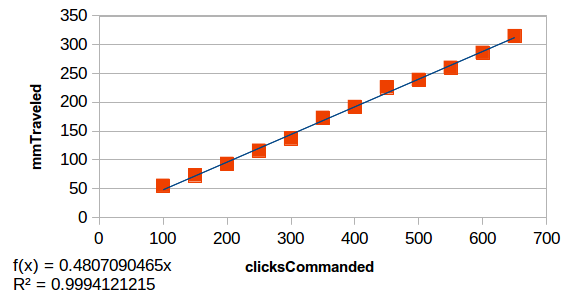
\includegraphics[width=0.8\linewidth]{motor_distance}
		\label{fig:motor_distance}
	}
	\hfill
	\subfloat[angle turned versus tacho counts (clicks) commanded] {
		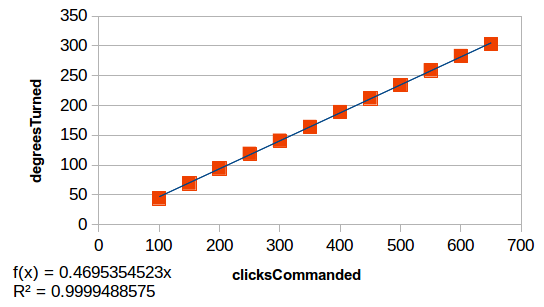
\includegraphics[width=0.8\linewidth]{rotation_distance}
		\label{fig:rotation_distance}
	}

	\label{fig:distance_testing}
	\caption{These are two plots generated by a series of commands where a movement metric was recorded as the result of a number of tacho counts (clicks) commanded.}

\end{figure}

\subsection{Odometry and Dead Reckoning}
Initially, a full dead reckoning system was attempted by following the calculations in ... . The resulting system worked but with too much error to be useful. Though we could've attempted to account for the error and make the system more accurate, the gain from having a working system didn't outweigh the cost of testing and developing it as we were able to complete the tasks without it.
Instead, it was settled on simply knowing the relation between wheel rotation and real-world distance and angular change. Through, testing (See section on testing) we were able to find a constant proportionality between the wheel rotations and distance travelled in millemeters and another for the wheel rotation and degrees turned using both wheels. These were useful especially in following the straight line tasks and object avoidance task as will be described later. 


\section{Methods}

\subsection{Tasks}

Each of the three tasks built upon each other, beginning with simple line following.

\subsubsection{Line following}

Our first solution to this problem was functional, but naive. We initiated a loop that operated by the following logic: if the robot was on the line (which could be determined by the value of the downward facing color sensor), turn right, otherwise, turn left. This resulted in the robot wiggling along the line with fairly wide turns and slow progress.

Then we revised our approach to use a PID controller instead. The overall idea was to set the goal of the PID controller to be the color/brightness value of the edge of the line. Therefore, the controller would constantly try to maintain that goal which would correspond to following the edge of the line. To normalize the readings fed to the PID controller, the raw readings from the color sensor had to undergo some calcultations. Firstly, the raw output of the color sensor was capped so that it's values stayed in the range of 10 and 50. Those values were then shifted accross by twenty so that they were centered across 0. Finally, the centered values were fed to the mathematical function tanh so that the values outputed were between -1 and 1. This information was sent as the current value to the PID each iteration. The goal of the PID was set to 0. Then, we did extensive tuning to achieve smooth results and steady-state accuracy.

Tuning the controller was an extensive process. We had to first scale the output of the PID controller to values that made sense to the motors. We set the base \code{duty\_cycle\_sp = 25} for each of the motors, so that when it had 0 error, it would move forward at 25\% speed.  So the output values had to be scaled to make sense for a change in motor power percentage. One motor's speed was increased and the other's decreased, or vice versa, based on the sign of the output.

Tuning process, and data from it.

For detecting when the robot has reached the end of the line, we used a combination of two features to make the judgment. We had a variable that incremented each iteration of the following loop if the robot was not on the line, and as soon as it was on the line again, then it was reset to 0. Thus, we could use this as essentially a time varaible tracking how long the robot has been looking for the line. If this number gets large it is likely the robot reached the end of the line. We also kept track of the difference in the robot's angle from the last time that it touched the line. If this difference got sufficiently large this also indicated the robot has been looking for the line for a while. Specifying these thresholds allowed us to break out of the loop when the robot was fairly sure it had reached the end of the line.

\subsubsection{Staggered line navigation}

\subsubsection{Obstacle avoidance}
\section{Testing}

\section{Results}

\section{Discussion}


\section*{Appendix}

\begin{verbatim}
	code
\end{verbatim}


\end{document}
